\section{Tool Calling} % (fold)
\label{sec:tool_calling}
%
\begin{frame}[t] \frametitle{Tool calling}
\framesubtitle{Descrizione}
{\footnotesize
\onslide<1->
    \begin{minipage}[t]{\textwidth}
        \begin{itemize}[leftmargin=10pt,align=right]
            \item[\alert{\faArrowCircleRight}] \textit{Design pattern} in AI (chiamata anche \textit{function calling})
            \item[\alert{\faArrowCircleRight}] Tecnica di mitigazione della \textit{knowledge cut-off}\ldots
            \item[\alert{\faArrowCircleRight}] \ldots ma non solo
            \onslide<2->\begin{itemize}[leftmargin=10pt,align=right]
                \item[\alert{\faArrowCircleRight}] Ricerca di informazioni non presenti nella sua base di conoscenza
                \begin{itemize}[leftmargin=10pt,align=right]
                    \item[\alert{\faArrowCircleRight}] ``Che tempo fa a Venezia?'' $\leadsto$ ``Soleggiato con temperature massime sui 20°C''
                    \onslide<3->\item[\alert{\faExclamationTriangle}] Quindi, differenza con RAG \textit{web search}...?!
                \end{itemize}
                \onslide<4->\item[\alert{\faArrowCircleRight}] Logica più semplice e mirata per recupero delle informazioni 
                \onslide<5->\item[\alert{\faArrowCircleRight}] Messa in atto di ciò che comprende
                \begin{itemize}[leftmargin=10pt,align=right]
                    \item[\alert{\faArrowCircleRight}] ``Prenota un biglietto'' $\leadsto$ \alert{\faTicket}
                    \item[\alert{\faArrowCircleRight}] ``Invia un'\textit{email}'' $\leadsto$ \alert{\faEnvelope}
                    \item[\alert{\faArrowCircleRight}] ``Fissa un appuntamento per martedì prossimo alle 18 in ufficio'' $\leadsto$ \alert{\faCalendar}
                \end{itemize}    
                \onslide<6->\item[\alert{\faArrowCircleRight}] Primo passaggio nella transizione da LLM a \alert{ALM} (Action Language Model)
            \end{itemize}
        \end{itemize}
    \end{minipage}
}
\end{frame}
%
\begin{frame}[t] \frametitle{Tool calling}
\framesubtitle{Differenze con RAG}
{\small
\onslide<1->
    \begin{minipage}[t]{\textwidth}
        {\footnotesize
            \begin{table}
                \renewcommand{\arraystretch}{1.3}
                \centering
                \begin{tabularx}{\textwidth}{p{5cm}p{5cm}}
                    \toprule
                    \textbf{RAG} & \textbf{\textit{Tool calling}}\\
                    \midrule
                     Leggere un manuale fai-da-te per risolverla da solo & Chiamare un idraulico per riparare una perdita\\
                    \midrule
                    ``In base a quello che mi hai chiesto e avendo letto alcuni documenti, ti spiego'' & ``In base a quello che mi hai chiesto, ecco come far agire il sistema con i mezzi a disposizione''\\
                    \midrule
                    Si concentra sulla generazione delle risposte utilizzando contenuti recuperati & Esegue azioni dal vivo o recupera dati dal vivo\\
                    \midrule                    
                    Recupera solo documenti e continua a generare la risposta & Richiede all'\textit{app client} di eseguire il \textit{tool}\\
                    \bottomrule
                \end{tabularx}
            \end{table}
        }
    \end{minipage}
}
\end{frame}
%
\begin{frame}[fragile,t] \frametitle{Tool calling}
\framesubtitle{Workflow in Spring AI - Default}
\vspace*{-.7cm}
{\footnotesize
    \begin{itemize}
        \only<1|handout:1>{\item[\alertedcircled{1}] L'utente invia la richiesta al LLM attraverso \texttt{ChatClient}/\texttt{ChatModel} riferendo al LLM i \textit{tool} a sua disposizione}
        \only<2|handout:2>{\item[\alertedcircled{2}] Se il LLM decide di chiamare un \textit{tool}, invia una \textit{response} con nome del \textit{tool} e parametri istanziati, seguendo la schema definito per il \textit{tool}}
        \only<3|handout:3>{\item[\alertedcircled{3}] L'applicativo inoltra all'effettiva implementazione del \textit{tool} nel \textit{container} Spring la richiesta con istanziazione dei parametri suggeriti dal LLM}
        \only<4|handout:4>{\item[\alertedcircled{4}] Il \textit{tool} esegue la sua logica di implementazione con i parametri restituiti dal LLM e restituisce il risultato al \textit{container} Spring}
        \only<5|handout:5>{\item[\alertedcircled{5}] Il sistema invoca nuovamente il LLM con la richiesta utente precedente ma ulteriormente contestualizzata dall'\textit{output} del \textit{tool}}
        \only<6|handout:6>{\item[\alertedcircled{6}] Il LLM restituisce la risposta finale al \texttt{ChatClient}/\texttt{ChatModel} sfruttando generazione di testo e contesto}
    \end{itemize}
    }
\vfill
\begin{figure}[ht]
    \centering
    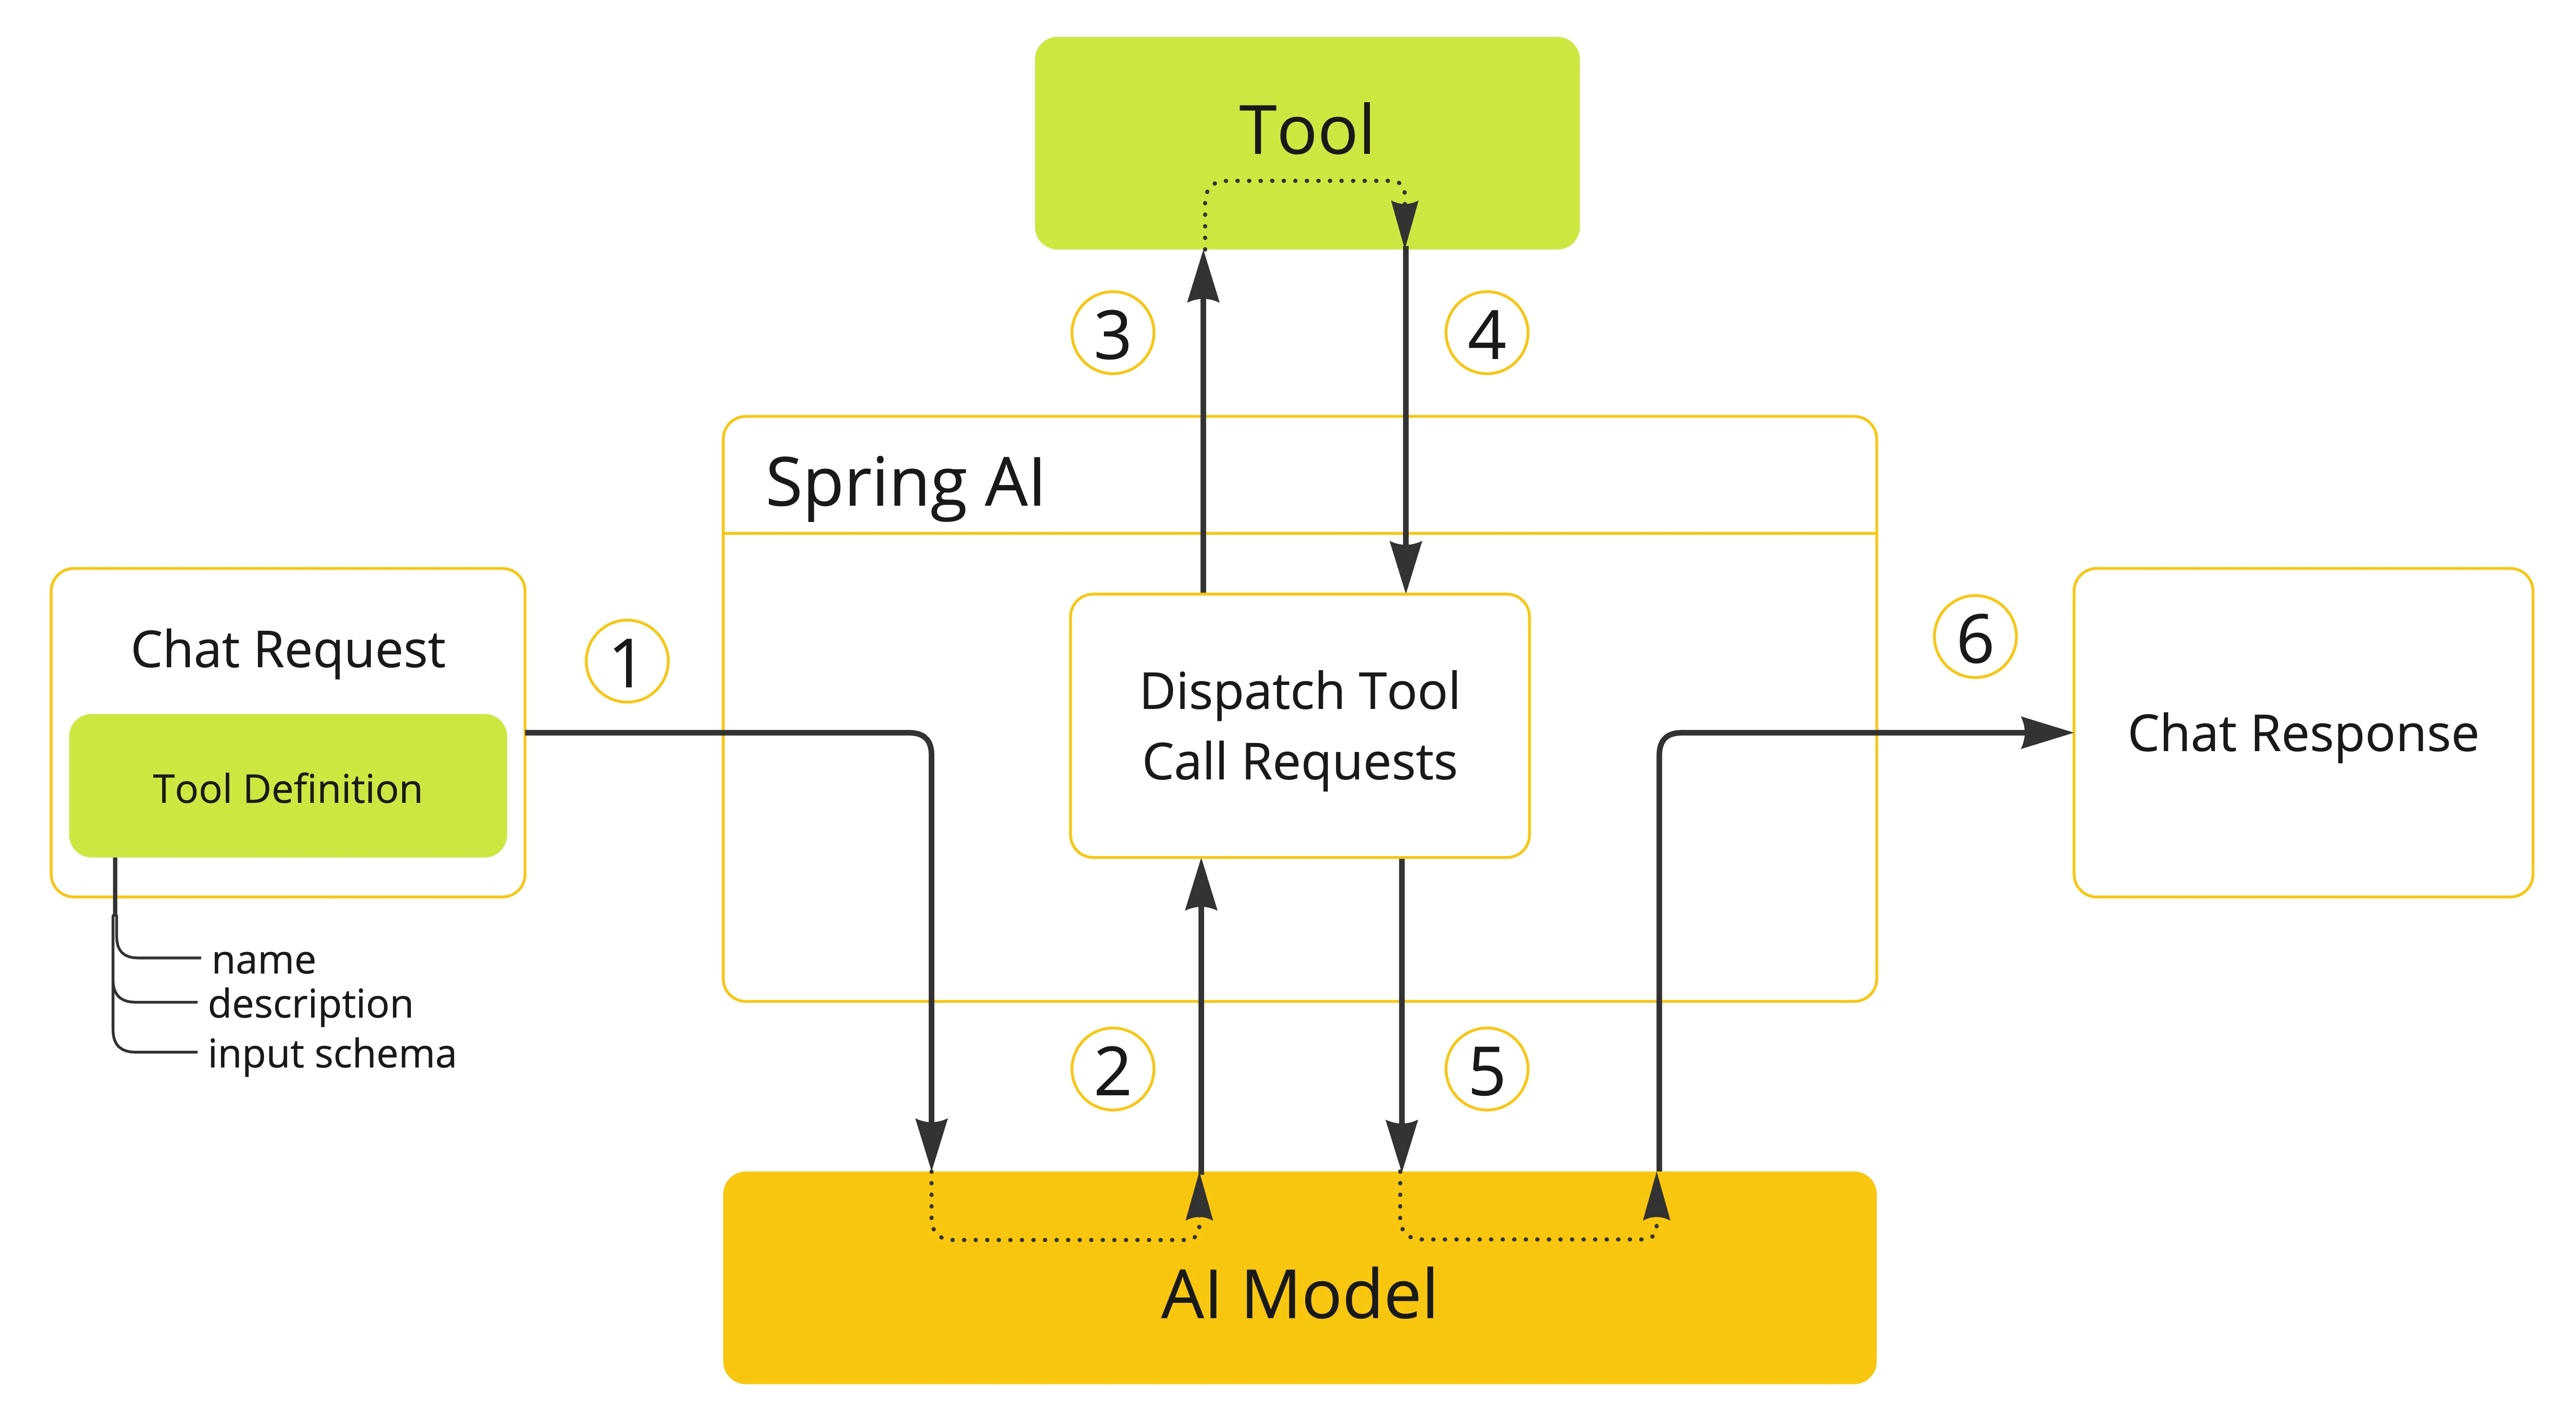
\includegraphics[width=\textwidth]{img/tool-calling.png}
    {\tiny\\\textit{\textcopyright Spring AI}}
\end{figure}
\end{frame}
%
\begin{frame}[fragile,t] \frametitle{Tool calling}
\framesubtitle{Workflow in Spring AI - Direct}
\vspace*{-.7cm}
{\footnotesize
    \begin{itemize}
        \only<1|handout:1>{\item[\alertedcircled{5}] Il sistema restituisce il risultato del \textit{tool} direttamente a \texttt{ChatClient}/\texttt{ChatModel} senza interrogare nuovamente il LLM}
    \end{itemize}
}
\vfill
\begin{figure}[ht]
    \centering
    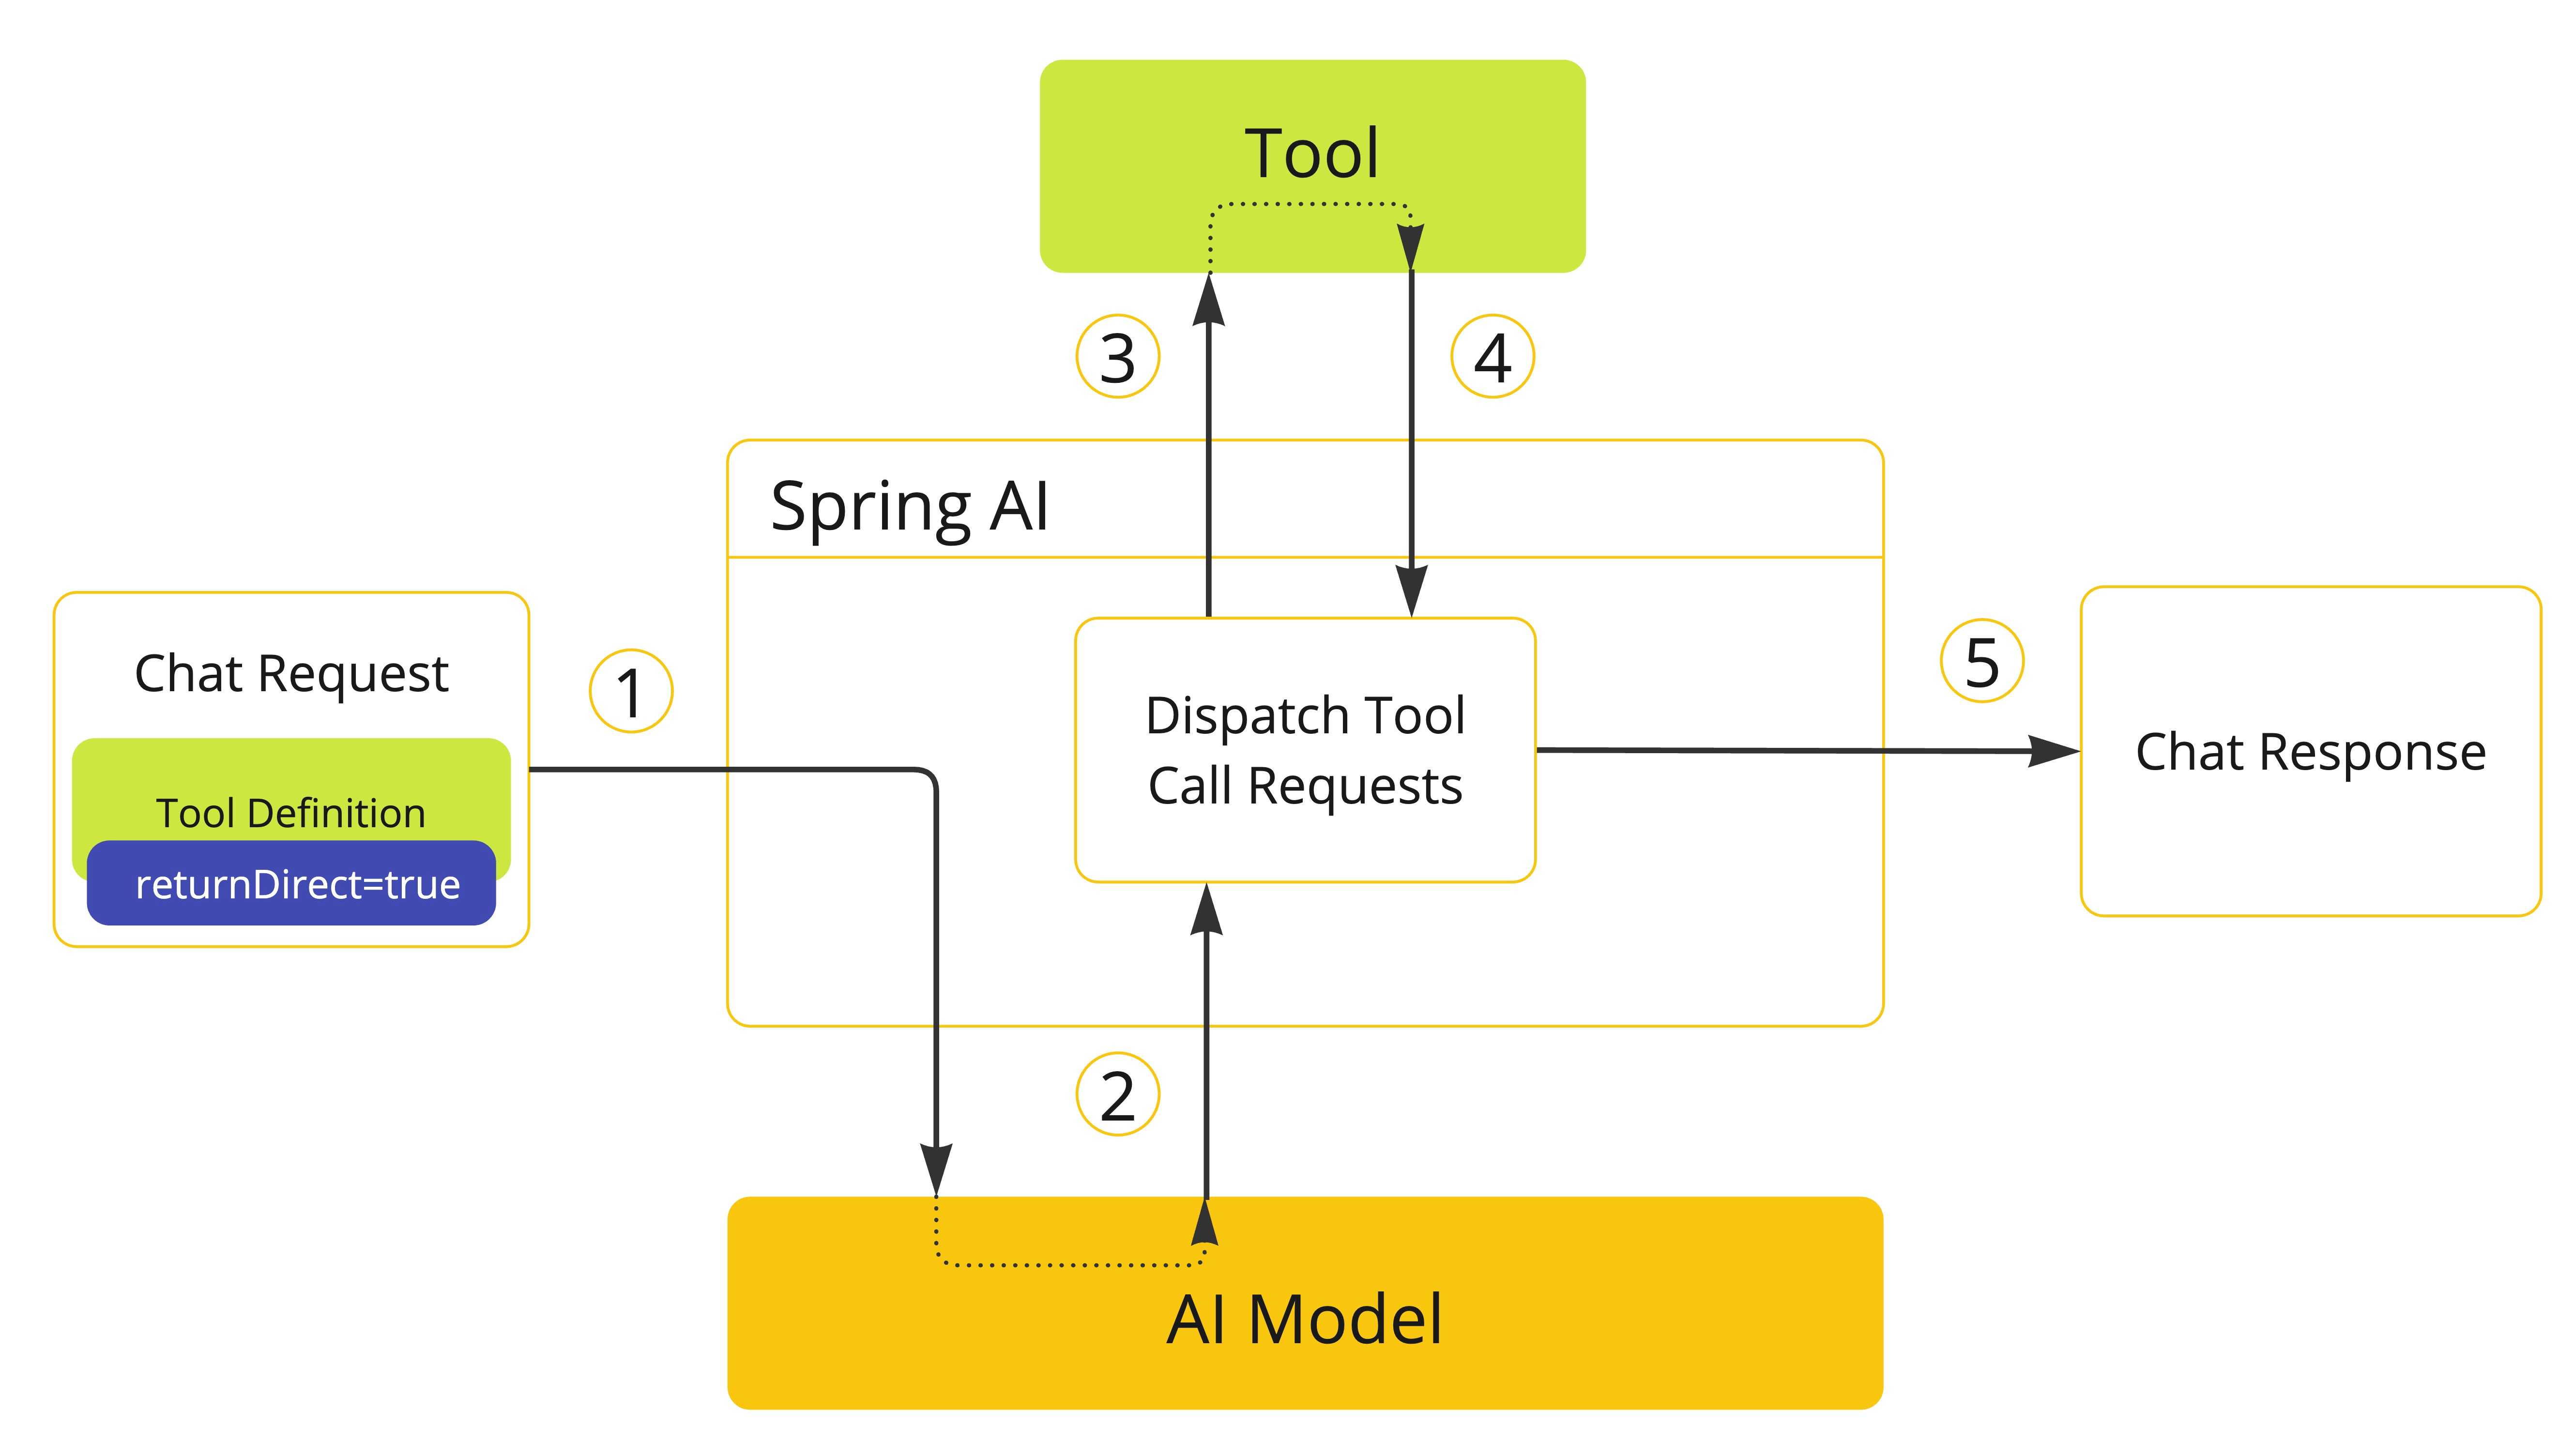
\includegraphics[width=\textwidth]{img/return-direct.png}
    {\tiny\\\textit{\textcopyright Spring AI}}
\end{figure}
\end{frame}
%
\begin{frame}[t] \frametitle{Tool calling}
\framesubtitle{Metodologie e paradigmi}
{\footnotesize
    \begin{minipage}[t]{\textwidth}
        \begin{itemize}[leftmargin=10pt,align=right]
            \onslide<1->\item[\alert{\faArrowCircleRight}] Metodologie
            \begin{itemize}[leftmargin=10pt,align=right]
                \onslide<2->\item[\alert{\faArrowCircleRight}] Dichiarativa 
                \onslide<3->\item[\alert{\faArrowCircleRight}] Programmatica
            \end{itemize}
            \onslide<1->\item[\alert{\faArrowCircleRight}] Paradigmi
            \begin{itemize}[leftmargin=10pt,align=right]
                \onslide<4->\item[\alert{\faArrowCircleRight}] \textit{\alert{M}ethod \alert{A}s \alert{T}ool} (\alert{MAT}) 
                \onslide<5->\item[\alert{\faArrowCircleRight}] \textit{\alert{F}unction \alert{A}s \alert{T}ool} (\alert{FAT})
            \end{itemize}
        \end{itemize}      
    \end{minipage}
}
\end{frame}
%
\section{Tool Calling\\\small{Method as tool}} % (fold)
\label{sec:tool_calling_mat}
%
\begin{frame}[fragile,t] \frametitle{MAT}
\framesubtitle{Spring AI - Approccio dichiarativo}
{\scriptsize
    \vspace*{-.8cm}
    \begin{minipage}[t]{\textwidth}
        \begin{block}{Classe di definizione dei \textit{tool}}
		    {\tiny\inputminted{java}{code/TimeTools.java}}
        \end{block}
        \only<2-4|handout:1>{
        \vspace*{.1cm}
        \begin{itemize}[leftmargin=10pt,align=right]
            \onslide<2->\item[\alert{\faArrowCircleRight}] Istanziati come \alert{\texttt{@Component}}
            \onslide<3->\item[\alert{\faArrowCircleRight}] Ogni metodo a disposizione del LLM come \textit{tool} deve essere annotato come \alert{\texttt{@Tool}}
            \onslide<4->\begin{itemize}[leftmargin=10pt,align=right]
                \item[\alert{\faArrowCircleRight}] se \texttt{name} non specificato, Spring AI popola il parametro con il nome del metodo
                \item[\alert{\faExclamationTriangle}] \texttt{name} come \alert{identificativo univoco} per Spring AI
                \item[\alert{\faArrowCircleRight}] \texttt{description} fornisce il \alert{contesto} al LLM per determinare se utilizzare il \textit{tool} in base alla richiesta utente!
                \item[\alert{\faArrowCircleRight}] \alert{\texttt{@ToolParam}} fornisce ulteriore contesto al LLM per iniettare parametri al metodo
                \item[\alert{\faArrowCircleRight}] \alert{\texttt{returnDirect}} per sovrascrivere il comportamento di \textit{default} se necessario 
            \end{itemize}
        \end{itemize}
        }
        \hspace*{2cm}
        \only<5|handout:2>{
        \begin{minipage}[t]{.8\textwidth}
			\renewcommand{\epigraphsize}{\scriptsize}
			\setlength{\afterepigraphskip}{5pt}
			\setlength{\beforeepigraphskip}{0pt}
			\setlength{\epigraphwidth}{\textwidth}
			\epigraph{\textit{\alert{\faUser} ``D: Che ore sono a New York?''\\
			\alert{\faTerminal\ (thinking)} --- Scansiono i tool a disposizione\ldots ---\\
            \alert{\faTerminal\ (thinking)} --- Vedo che ho dei tool che gestiscono il recupero dell'ora\ldots ---\\
            \alert{\faTerminal\ (thinking)} --- Il primo tool è relativo alla posizione dell'utente\ldots ---\\
            \alert{\faTerminal\ (thinking)} --- Il secondo tool è più astratto e determina la posizione attraverso parametrizzazione del fuso orario\ldots ---\\
            \alert{\faTerminal\ (thinking)} --- \ldots Il fuso orario di New York è America/New York\ldots ---\\
			\alert{\faTerminal} ``R: Utilizza il tool \texttt{getCurrentTime('America/New York')}.''}}{\textbf{Processo di \textit{method as tool}}}
        \end{minipage}
        }
    \end{minipage}
}
\end{frame}
%
\begin{frame}[fragile,t] \frametitle{MAT}
\framesubtitle{Spring AI - Approccio dichiarativo}
{\footnotesize
    \vspace*{-.7cm}
    \begin{minipage}[t]{\textwidth}
        \begin{block}{\textit{Tool-aware} \texttt{ChatClient} - approccio statico}
		    {\tiny\inputminted{java}{code/TimeToolsConfig.java}}
        \end{block}
        \begin{block}{\textit{Tool-aware} \texttt{ChatClient} - approccio dinamico}
		    {\tiny\inputminted{java}{code/TimeToolsServiceImpl.java}}
        \end{block}
    \end{minipage}
}
\end{frame}
%
\begin{frame}[fragile,t] \frametitle{MAT}
\framesubtitle{Spring AI - Approccio programmatico}
{\scriptsize
    \vspace*{-.8cm}
    \begin{minipage}[t]{\textwidth}
        \begin{block}{Classe di definizione dei \textit{tool}}
		    {\tiny\inputminted{java}{code/TimeTools-2.java}}
        \end{block}
        \vspace*{.3cm}
        \begin{itemize}[leftmargin=10pt,align=right]
            \item[\alert{\faArrowCircleRight}] \alert{\texttt{@ToolParam}} permesso in approccio sia dichiarativo che programmatico
        \end{itemize}
    \end{minipage}
}
\end{frame}
%
\begin{frame}[fragile,t] \frametitle{MAT}
\framesubtitle{Spring AI - Approccio programmatico}
{\scriptsize
    \vspace*{-.8cm}
    \begin{minipage}[t]{\textwidth}
        \begin{block}{Utilizzo approccio \textit{method-tool callback}}
		    {\tiny\inputminted{java}{code/MethodToolCallback.java}}
        \end{block}        
        \vspace*{.1cm}
        \begin{itemize}[leftmargin=10pt,align=right]
            \onslide<2->\item[\alert{\faArrowCircleRight}] Il sistema usa \textit{reflection} per linkare il metodo 
            \onslide<3->\item[\alert{\faArrowCircleRight}] Costruito un \alert{\texttt{ToolCallback}} che definisce la logica di utilizzo del \textit{tool}
            \begin{itemize}[leftmargin=10pt,align=right]
                \item[\alert{\faArrowCircleRight}] \alert{\texttt{ToolDefinitions.Builder}} permette di definire nome, descrizione e schema del \textit{tool}
                \item[\alert{\faArrowCircleRight}] \alert{\texttt{ToolMetadata.Builder}} responsabile della definizione strategia \textit{default vs direct}
            \end{itemize}  
            \onslide<4->\item[\alert{\faExclamationTriangle}] Definizione \alert{\texttt{ToolCallback}} \textit{under-the-hood} anche con approccio dichiarativo
        \end{itemize}
    \end{minipage}
}
\end{frame}
%
\begin{frame}[fragile,t] \frametitle{MAT}
\framesubtitle{Spring AI - Approccio programmatico}
{\footnotesize
    \vspace*{-.7cm}
    \begin{minipage}[t]{\textwidth}
        \begin{block}{\textit{Tool-aware} \texttt{ChatClient} - approccio statico}
		    {\tiny\inputminted{java}{code/ToolConfig-2.java}}
        \end{block}
        \begin{block}{\textit{Tool-aware} \texttt{ChatClient} - approccio dinamico}
		    {\tiny\inputminted{java}{code/TimeToolsServiceImpl-2.java}}
        \end{block}
    \end{minipage}
}
\end{frame}
%
\begin{frame}[fragile,t] \frametitle{MAT}
\framesubtitle{Vincoli Spring AI}
{\footnotesize
    \begin{minipage}[t]{\textwidth}
        \begin{itemize}[leftmargin=10pt,align=right]
            \onslide<1->\item[\alert{\faArrowCircleRight}] \alert{Restrizioni di tipo} per parametri e valori di ritorno
            \onslide<2->\item[\alert{\faExclamationTriangle}] Tipi non supportati
            \begin{itemize}[leftmargin=10pt,align=right]
                \onslide<3->\item[\alert{\faArrowCircleRight}] \textbf{Tipi Optional} - \texttt{Optional<T>} non è compatibile
                \onslide<4->\item[\alert{\faArrowCircleRight}] \textbf{Costrutti asincroni} - \texttt{CompletableFuture}, \texttt{Future}
                \onslide<5->\item[\alert{\faArrowCircleRight}] \textbf{Tipi reattivi} - \texttt{Flow}, \texttt{Mono}, \texttt{Flux}
                \onslide<6->\item[\alert{\faArrowCircleRight}] \textbf{Tipi funzionali} - \texttt{Function}, \texttt{Supplier}, \texttt{Consumer}
            \end{itemize}
            \onslide<7->\item[\alert{\faExclamationTriangle}] I tipi funzionali sono supportati attraverso l'approccio \alert{function-based} dedicato
        \end{itemize}
    \end{minipage}
}
\end{frame}
%
\section{Tool Calling\\\small{Function as tool}} % (fold)
\label{sec:tool_calling_fat}
%
\begin{frame}[fragile,t] \frametitle{FAT}
\framesubtitle{Spring AI - Approccio dichiarativo}
{\scriptsize
    \vspace*{-.7cm}
    \begin{minipage}[t]{\textwidth}
        \begin{block}{Classe di definizione dei \textit{tool}}
		    {\tiny\inputminted{java}{code/WeatherTools.java}}
        \end{block}
        \vspace*{.3cm}
        \begin{itemize}[leftmargin=10pt,align=right]
            \onslide<1->\item[\alert{\faExclamationTriangle}] \textbf{Tipi funzionali supportati:} \texttt{Function<I,O>}, \texttt{Supplier<O>}, \texttt{Consumer<I>}, \texttt{BiFunction<I1,I2,O>}
            \onslide<2->\item[\alert{\faArrowCircleRight}] Ciascun funzionale disponibile come \textit{tool} attraverso definizione \alert{\texttt{@Bean}}
            \begin{itemize}[leftmargin=10pt,align=right]
                \item[\alert{\faExclamationTriangle}] Definire nome come \alert{costante esportabile} per mancanza di garanzia \textit{type safety}
            \end{itemize}
            \onslide<3->\item[\alert{\faArrowCircleRight}] \alert{\texttt{@Description}} come \texttt{description} di MAT
            \onslide<4->\item[\alert{\faArrowCircleRight}] \alert{\texttt{@ToolParam}} con medesima logica di MAT
        \end{itemize}
    \end{minipage}
}
\end{frame}
%
\begin{frame}[fragile,t] \frametitle{FAT}
\framesubtitle{Spring AI - Approccio dichiarativo}
{\footnotesize
    \vspace*{-.7cm}
    \begin{minipage}[t]{\textwidth}
        \begin{block}{\textit{Tool-aware} \texttt{ChatClient} - approccio statico}
		    {\tiny\inputminted{java}{code/WeatherToolsConfig.java}}
        \end{block}
        \begin{block}{\textit{Tool-aware} \texttt{ChatClient} - approccio dinamico}
		    {\tiny\inputminted{java}{code/WeatherToolsServiceImpl.java}}
        \end{block}
    \end{minipage}
}
\end{frame}
%
\begin{frame}[fragile,t] \frametitle{FAT}
\framesubtitle{Spring AI - Approccio programmatico}
{\scriptsize
    \vspace*{-.8cm}
    \begin{minipage}[t]{\textwidth}
        \begin{block}{Classe di definizione dei funzionali}
		    {\tiny\inputminted{java}{code/TemperatureService.java}}
        \end{block}
        \vspace*{.3cm}
        \begin{itemize}[leftmargin=10pt,align=right]
            \item[\alert{\faArrowCircleRight}] Richiesta sola la logica pertinente al funzionale scelto (es. \texttt{apply} per \texttt{Function})
        \end{itemize}
    \end{minipage}
}
\end{frame}
%
\begin{frame}[fragile,t] \frametitle{FAT}
\framesubtitle{Spring AI - Approccio programmatico}
{\scriptsize
    \vspace*{-.8cm}
    \begin{minipage}[t]{\textwidth}
        \begin{block}{Utilizzo approccio \textit{function-tool callback}}
		    {\tiny\inputminted{java}{code/FunctionToolCallback.java}}
        \end{block}        
        \vspace*{.1cm}
        \begin{itemize}[leftmargin=10pt,align=right]
            \onslide<2->\item[\alert{\faArrowCircleRight}] \texttt{FunctionToolCallback.Builder} linka un identificativo testuale ad una istanza di una nuova \textit{function tool}
            \onslide<3->\item[\alert{\faArrowCircleRight}] Costruito un \alert{\texttt{ToolCallback}} che definisce la logica di utilizzo del \textit{tool}
            \begin{itemize}[leftmargin=10pt,align=right]
                \item[\alert{\faArrowCircleRight}] \alert{\texttt{ToolDefinitions.Builder}} permette di definire nome, descrizione e schema del \textit{tool}
                \item[\alert{\faArrowCircleRight}] \alert{\texttt{ToolMetadata.Builder}} responsabile della definizione strategia \textit{default vs direct}
            \end{itemize}  
            \onslide<4->\item[\alert{\faExclamationTriangle}] Definizione \alert{\texttt{ToolCallback}} \textit{under-the-hood} anche con approccio dichiarativo
        \end{itemize}
    \end{minipage}
}
\end{frame}
%
\begin{frame}[fragile,t] \frametitle{FAT}
\framesubtitle{Spring AI - Approccio programmatico}
{\footnotesize
    \vspace*{-.7cm}
    \begin{minipage}[t]{\textwidth}
        \begin{block}{\textit{Tool-aware} \texttt{ChatClient} - approccio statico}
		    {\tiny\inputminted{java}{code/WeatherToolsConfig-2.java}}
        \end{block}
        \begin{block}{\textit{Tool-aware} \texttt{ChatClient} - approccio dinamico}
		    {\tiny\inputminted{java}{code/WeatherToolsServiceImpl-2.java}}
        \end{block}
    \end{minipage}
}
\end{frame}
%